\section{Proposed software architecture}
\subsection{Overview}
The following chapter will go through: the chosen architecture patterns and design of the calendar system, the design patterns used to implement it and how the control flow of the program.
\subsection{Subsystem decomposition}
The figure below shows the subsystem decomposition of the User part of the program.
\begin{figure}[h]
\centering
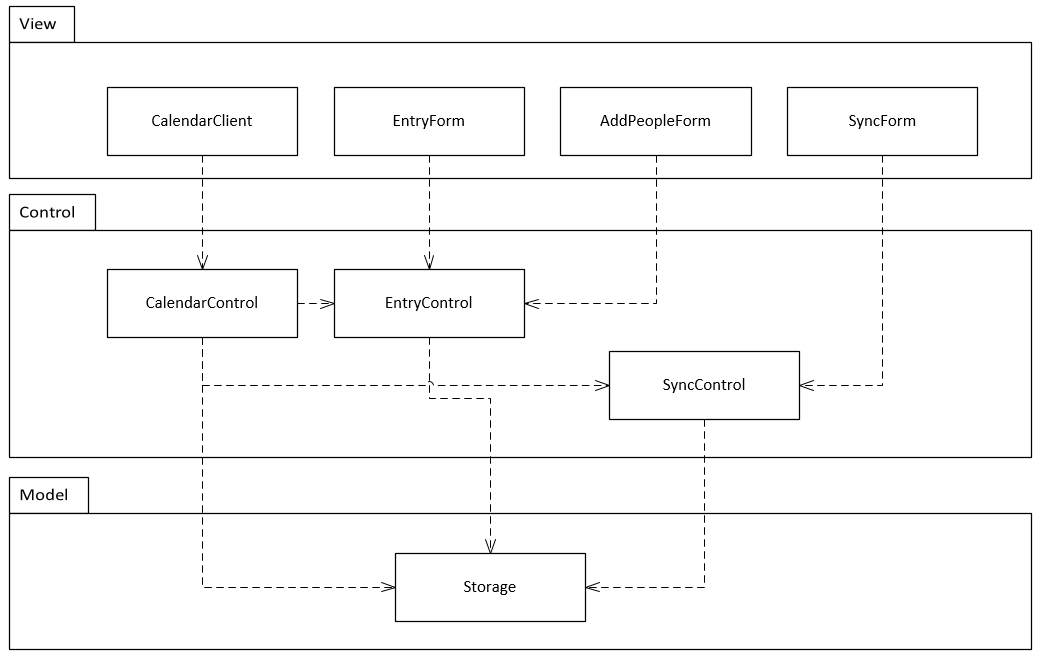
\includegraphics[scale = 0.6]{systemModel}
\caption{Subsystems and their decomposition}
\end{figure}
\subsection{Hardware/software mapping}
\subsection{Persistent data management}
The two kinds of objects the Calendar System is meant to store are Users and Entries. The Entries will be available for to create and modify for Users, while the Users can only be created and modified by an administrator. Thus we will need to kinds of access controls\footnote{see: Access control and security}. The storage system will provide an interface that enables the usage of three different kinds of storage: Online storage (will be implemented as a relational database), offline storage (will be implemented using serialization) and a test storage with no persistence for testing purposes only.
\subsection{Access control and security}
There are only two kinds of actors that will be using the Calendar System: User and Administrator. Everyone using the system will have a User account including the administrators, although they will have added priveledges. When creating or modifying an account you will have to specify whether or not this user should have administrator priveledges also.
\subsection{Global software control}
\subsection{Boundary conditions}